% !TeX spellcheck = pl_PL
\documentclass[a4paper,twoside]{article}
\usepackage{polski}
\usepackage[utf8]{inputenc}
\usepackage[pdftex]{graphicx}
\usepackage{amsmath}

\usepackage[unicode, bookmarks=true]{hyperref} %do zakładek
\usepackage{tabto} % do tabulacji
\NumTabs{6} % globalne ustawienie wielkosci tabulacji
\usepackage{array}
\usepackage{multirow}
\usepackage{array}
\usepackage{dcolumn}
\usepackage{bigstrut}
\usepackage{color}
\usepackage[usenames,dvipsnames]{xcolor}
\usepackage{pdfpages}
\usepackage{sidecap}
\usepackage{wrapfig}
\usepackage{float}	%for figure& table placement in text


\setlength{\textheight}{24cm}
\setlength{\textwidth}{15.92cm}
\setlength{\footskip}{10mm}
\setlength{\oddsidemargin}{0mm}
\setlength{\evensidemargin}{0mm}
\setlength{\topmargin}{0mm}
\setlength{\headsep}{5mm}
\newcommand{\HRule}{\rule{\linewidth}{0.5mm}} 

\newcolumntype{M}[1]{>{\centering\arraybackslash}m{#1}}
\newcolumntype{N}{@{}m{0pt}@{}}

\graphicspath{ {./img/} }

% === Reset inkrementacji sekcji przy nowym parcie === %
\usepackage{titlesec}

\makeatletter
\@addtoreset{section}{part}
\makeatother
\titleformat{\part}[display]
{\normalfont\LARGE\bfseries\left}{}{0pt}{}

\titleformat{\chapter}[hang]{\LARGE\bfseries}{\thechapter\hsp\textcolor{blue}{|}\hsp}{0pt}{\Huge\bfseries}


\begin{document}
	
	\begin{titlepage}
		\begin{center}
			
			% Upper part of the page. The '~' is needed because \\
			% only works if a paragraph has started.
			
\includegraphics[width=0.5\textwidth]{./img/logo.png}~\\[1cm]
			%?[width=0.15\textwidth]
			
			\textsc{\LARGE Politechnika Śląska w Gliwicach}\\[1.5cm]
			
			\textsc{\Large Przemysłowe systemy rozproszone}\\[0.5cm]
			
			% Title
			\HRule \\[0.4cm]
			{ \huge \bfseries Protokoły dostępu do łącza stosowane w sieciach przemysłowych. Sieci o dostępie typu Master-Slave. Zachowanie reguł determinizmu czasowego.  \\[0.4cm] }
			
			\HRule \\[1.5cm]
			
			% Author and supervisor
			\textsc{\Large Autorzy:} \\
			Bartłomiej Buchała \\
			Mateusz Forczmański\\
			
			\vfill
			
			% Bottom of the page
			{\large \today}
			
		\end{center}
	\end{titlepage}
	
\newpage

\section{\textcolor{blue}{Wstęp}}

Wraz z rozwojem informatyki, znalazła ona szerokie zastosowanie w różnych gałęziach przemysłu.  Zastosowanie systemu informatycznego niesie ze sobą wiele korzyści, m. in: \\
\begin{itemize}
	\item Automatyzacja wykonywanych czynności \\
	\item Przyspieszenie obliczeń \\
	\item Autokorekcja w przypadku, kiedy dojdzie do częściowej awarii systemy \\
\end{itemize}

Przy stosunkowo niewielkim koszcie (zaprojektowanie, zaprogramowanie, instalacja takiego systemu).  Problem pojawił się przy dalszej rozbudowie branży przemysłowej (co dla części informatycznej oznaczało przede wszystkim rosnącą złożoność obliczeniową zastosowanych algorytmów czy większą liczbę urządzeń do obsłużenia). Dodatkowo, pewnym utrudnieniem jest mniejsza w ostatnich latach dynamika rozwoju mocy obliczeniowej pojedynczych komputerów, co jest związane ze zbliżaniem się do pułapu miniaturyzacji elementów. Remedium na ten problem okazało się zastosowanie \textbf{systemów rozproszonych czasu rzeczywistego.} \\

Dla systemu czasu rzeczywistego, oprócz warunków logicznych, ważne jest również spełnienie warunków czasowych. Oznacza to, że oprócz poprawnych rezultatów musi on również zapewnić ich wykonanie w odpowiednim czasie. Można wyróżnić systemy czasu rzeczywistego, które tolerują przekroczenie ograniczeń czasowych (interwału czasowego), i takie dla których czas operacji jest wartością krytyczną. \\

Podstawową cechą systemów rozproszonych jest fakt, że jest to zbiór niezależnych od siebie komputerów (lub rzadziej procesorów, jeżeli mówimy o komputerach wieloprocesorowych), połączonych siecią komputerową. Posiadają one wspólne oprogramowanie, które pozwala im na współdziałanie (podział zasobów, współbieżne wykonywanie obliczeń) w określonym przez twórcę celu. Komputery będące elementami większego systemu rozproszonego najczęściej nazywa się \textbf{węzłami}. Aby zapewnić poprawną pracę, wymagana jest odpowiednia komunikacja między węzłami.

\section{\textcolor{blue}{Struktura węzła w sieci przemysłowej}}
Rolę węzła systemu rozproszonego najczęściej pełni sterownik swobodnie programowalny (PLC) lub grupa takich sterowników.  PLC jest uniwersalnym urządzeniem mikroprocesorowym, którego zadaniem jest sterowanie maszyną lub urządzeniem technicznym. Realizuje on program znajdujący się w jego pamięci operacyjnej. Ponieważ węzeł jest elementem większej sieci, samo PLC nie wystarcza. Zazwyczaj pojedynczy moduł ma budowę trójwarstową: \\

\begin{center}
	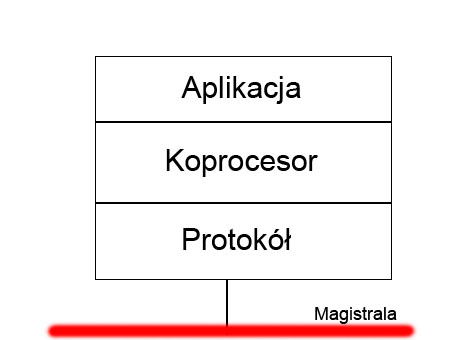
\includegraphics[width=8cm]{./img/wezel.jpg}
\end{center}

\begin{itemize}
	\item Przez \textbf{aplikację} rozumiemy znajdujący się w sterowniku PLC system operacyjny czasu rzeczywistego oraz program cyklicznie realizujący określone przez programistę założenia. Ten poziom odpowiada za faktyczną pracę urządzenia i jest częściowo niezależny od innych węzłów systemu. \\
	\item \textbf{Koprocesor} jest elementem pracującym niezależnie od głównego procesora urządzenia. Jest on odpowiedzialny za komunikację pomiędzy macierzystym układem, a siecią. Posiada dwa zastosowania: 
	\begin{itemize}
		\item Nadawanie – otrzymując informacje od procesora głównego,  kopiuje ona odpowiednie fragmenty pamięci do buforów nadawczych, następnie transformuje je do odpowiedniej formy (ramki transmisyjne), po czym wysyła je przy użyciu nadajnika (portu UART) \\
		\item Odbieranie – przechwytuje informacje z sieci skierowane do tego węzła i dekoduje je do formy mogącej być odczytaną przez sterownik. Po tym następuje skopiowanie treści do bufora odbiorczego i przepisanie do pamięci urządzenia 
	\end{itemize}
	\item Protokół transmisji jest ściśle związany z koprocesorem sieci. Jest zbiorem zasad, na jakich odbywa się połączenie pomiędzy dwoma lub więcej węzłami w sieci. Dzięki temu możliwa jest komunikacja sterowników działających na różnym oprogramowaniu. \\
	
\end{itemize}

W dalszej części wypracowania skupimy się głównie na tym ostatnim.


\section{\textcolor{blue}{Rodzaje protokołów stosowane w sieciach przemysłowych}}

Ponieważ rozproszona sieć przemysłowa czasu rzeczywistego powinna się charakteryzować  skończonym czasem przekazywania danych, będą nas interesować jedynie protokoły o zdefiniowanym (deterministycznym) w czasie dostępie. 

\end{document}